\chapter{Analyse \& Design ( 25 \%)}






\section{\"Uberblick}
\subsection{Hauptkomponenten}

\subsection{Grundlegendes Datenmodell}

\section{Vorbereitende Primitiven}
\subsection{watch\_for}
\subsection{run\_callbacks}

\section{Projektkonfiguration}

\section{Auftragsannahme}

\begin{figure}[ht] 
  \label{fig:lebenszyklus-auftrag-eingang}
  \begin{center}
      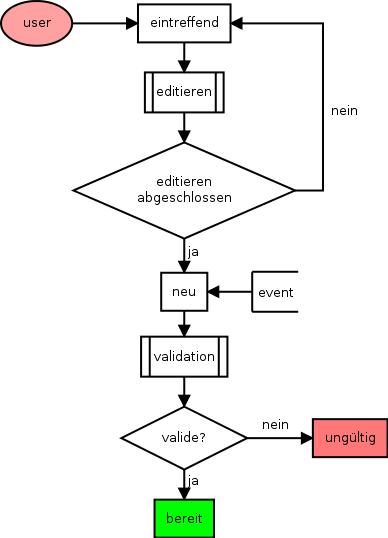
\includegraphics[height=5in]{imageinput/lebenszyklus-auftrag-eingang.png}
  \end{center}
  \caption{Auftragsannahme: Flowgraph}
\end{figure}


\subsection{Eingang}
\subsection{Validation}

\section{Management}



\begin{figure}[ht] 
  \label{fig:lebenszyklus-auftrag-abarbeitung}
  \begin{center}
      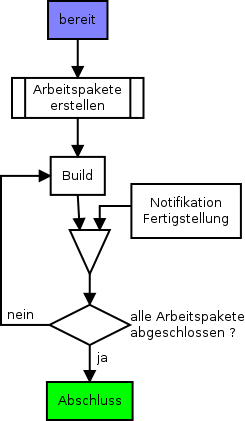
\includegraphics[height=4in]{imageinput/lebenszyklus-auftrag-abarbeitung.png}
  \end{center}
  \caption{Auftragsannahme: Flowgraph}
\end{figure}

\subsection{Auftragsvorbereitung}
\subsection{Bereitstellung von Arbeitspacketen}
\subsection{Abschluss von auftr\"agen}


\section{Zuteilung/Abarbeitung von Arbeitspacketen}
\subsection{Zuteilungs}
\subsection{Vorbereitung Abarbeitung}
\subsection{Abschluss Abarbeitung}


\section{Abarbeitung von Arbeitspacketen}
\subsection{Arbeitsschritte}
\subsection{Datensammlung zur Laufzeit}
\subsection{Datensammling nach Abschluss eines Schrittes}
\subsection{Abschluss von Arbeitschritten}


\section{Arten von Arbeitschritten}
\subsection{Prozessaktionen}
\subsection{Quellcode Management Aktionen}
\subsection{Theoretische Betrachtung Interaktion}
